% Provenance (never printed): see sources/outline_sources.md (Year 2: humidity variables;
% Clausius--Clapeyron applied; dry and moist adiabats; thermodynamic diagrams; convective
% instability; cloud microphysics). Definitions after the NWS glossary; skew-T lines, CAPE classes
% and the lifted index after the NWS Houston/Galveston training page; saturation data from the
% NIST WebBook (IAPWS-95) and IAPWS R14-08; the empirical formula as used by Su and others
% (2026); kappa-Koehler theory after Petters and Kreidenweis (2007); CCN numbers after Andreae
% (2009); the processes of microphysics after Morrison and others (2020). The sounding is the
% real 12 UTC sounding of Norman, Oklahoma, 16 April 2026 (IGRA2); every curve and number from
% figdata/bachelor-2/thermo.py; exercise and problem values in the Book 4 scratch calculator
% calc/ch21.py.
\chapter{الديناميكا الحرارية للغلاف الجوي}\label{ch:b2:atmospheric-thermodynamics}

في 16 أبريل 2026، عند الساعة 12 بالتوقيت العالمي المنسّق، ارتفع منطاد من محطّة الأرصاد في نورمان، أوكلاهوما، كما
ترتفع المناطيد من أكثر من ثمانمئة محطّة في تلك الساعة كلّ يوم. وأرسل الجهاز الذي
حمله لاسلكيًّا مقطعًا رأسيًّا يقرؤه المتنبّئ بنظرة: هواء قرب الأرض
مشبع تقريبًا، وغطاء دافئ رقيق على ارتفاع ستّمئة متر، وفوقه حرارة تنخفض
بسرعة على مدى عشرة كيلومترات. ولو رُفع هواء السطح عبر الغطاء، لوجد نفسه
أدفأ من محيطه في معظم التروبوسفير، ومعه نحو ألفي جول لكل
كيلوغرام ينفقها في الصعود. يتعلّم هذا الفصل قراءة تلك الطاقة من سبر جوّي: كم من
الماء يحمل الهواء، وكيف يبرد طرد صاعد قبل أن يتكاثف وبعده، وكيف تحوّل مخطّطات
علماء الأرصاد المساحاتِ إلى طاقات، وكيف تتكوّن قطيرات السحاب أصلًا.
% ledger: data:b4-sounding, nws4:upperair, nws4:cape

\begin{recall}
\textbf{من كتب الفيزياء}: \omterm{def:b2:atmospheric-thermodynamics:moist-air}{ضغط البخار} المشبع، والرطوبة النسبية، ونقطة الندى،
والحرارة الكامنة، وعلاقة كلاوزيوس--كلابيرون وصيغتها المكاملة؛ والتنوّي
وفرط التبريد؛ والقانون الأول، والتحوّلات الأديباتية والسعات الحرارية للغاز المثالي.
\textbf{من كتب الكيمياء}: الضغوط الجزئية، وقانون راؤول، والتوتّر السطحي ومعادلة
كلفن. \textbf{من مجلّدات المدرسة}: \omterm{def:b2:atmospheric-thermodynamics:lcl}{مستوى التكاثف} وقاعدته
\qty{125}{m} لكل درجة، والهواء المستقرّ وغير المستقرّ، \omterm{def:b2:atmospheric-thermodynamics:microphysics}{ونواة التكاثف}، وآليتا المطر الدافئ
والبلورات الجليدية. \textbf{من مجلد السنة الأولى}: الغلاف الجوي المعياري، ومعدّل الانخفاض البيئي
ومعدّل الانخفاض الأديباتي الجاف ($\Gamma_d = \qty{9.8}{K/km}$)، والطرد الهوائي، ودرجة الحرارة
الكامنة، والاستقرار الساكن، والانعكاسات الحرارية والمعادلة الهيبسومترية.
\end{recall}

في الفصل كلّه: $R_d = R/M_d = \qty{287.0}{J.kg^{-1}.K^{-1}}$ للهواء الجاف ذي الكتلة المولية
\qty{28.97}{g/mol}؛ و$R_v = R/M_w = \qty{461.5}{J.kg^{-1}.K^{-1}}$ لبخار الماء، ذي الكتلة
المولية \qty{18.0153}{g/mol}؛ و$\varepsilon = M_w/M_d = 0.622$؛ و$c_p = \tfrac72 R_d =
\qty{1004.5}{J.kg^{-1}.K^{-1}}$ (مجلد السنة الأولى، مع نسبة السعتين الحراريتين 1.4)؛
و$g = \qty{9.81}{m.s^{-2}}$؛ والحرارة الكامنة للتبخّر عند النقطة الثلاثية،
$L = \qty{2.501e6}{J/kg}$.
% ledger: const:R, earth:Mmol, nist4:water-mw, nasa:grc-gamma, const:gn, nist4:water-sat

\section{الهواء الرطب}\label{sec:b2:atmospheric-thermodynamics:moist-air}

الهواء مزيج من الهواء الجاف وبخار الماء، وكلاهما قريب من الغاز المثالي. وتقيس كتب الفيزياء
ماءه بالرطوبة النسبية ونقطة الندى؛ أمّا الطرد الصاعد فيحتاج إلى مقاييس
لا تتغيّر حين يتمدّد.

\begin{definition}[ضغط البخار؛ نسبة الخلط؛ الرطوبة النوعية]\label{def:b2:atmospheric-thermodynamics:moist-air}
\emph{ضغط البخار}\index{ضغط البخار} $e$ للهواء الرطب هو الضغط الجزئي
لبخار مائه. و\emph{نسبة الخلط}\index{نسبة الخلط} له هي $r = m_v/m_d$، أي كتلة بخار
الماء لكل وحدة كتلة من الهواء الجاف في الحجم نفسه، و\emph{الرطوبة
النوعية}\index{الرطوبة النوعية} له هي $q = m_v/(m_d + m_v)$، أي كتلة البخار لكل وحدة كتلة من
الهواء الرطب. وكلتاهما تُعطى عادة بالغرامات لكل كيلوغرام.
\end{definition}
% ledger: nws4:humidity

\begin{proposition}[متغيّرات الرطوبة]\label{prop:b2:atmospheric-thermodynamics:humidity}
في هواء رطب عند الضغط الكلّي $p$ \omterm{def:b2:atmospheric-thermodynamics:moist-air}{وضغط البخار} $e$،
\[
  r = \frac{\varepsilon e}{p - e}, \qquad q = \frac{r}{1 + r} = \frac{\varepsilon e}{p - (1 -
  \varepsilon)e} .
\]
عند التشبّع، $e = e_s(T)$ و$r = r_s(T, p)$، وهي \omterm{def:b2:atmospheric-thermodynamics:moist-air}{نسبة الخلط} المشبعة. ولا تتغيّر $r$ ولا
$q$ حين يتمدّد طرد أو ينضغط دون أن يكسب ماءً أو يفقده.
\end{proposition}

\begin{proof}
في الحجم نفسه $V$ وعند درجة الحرارة $T$، يخضع كلّ غاز لقانون الغاز المثالي الخاصّ به مع
ضغطه الجزئي: $m_v = eV/(R_vT)$ و$m_d = (p - e)V/(R_dT)$، فيكون $r = (R_d/R_v)\,e/(p - e)$،
و$R_d/R_v = M_w/M_d = \varepsilon$. وقسمة $m_v$ على $m_d + m_v$ تعطي $q = r/(1 + r)$.
والتمدّد يغيّر $V$ و$p$ و$e$ لكنه لا يغيّر الكتلتين.
\end{proof}

\begin{definition}[درجة الحرارة الافتراضية]\label{def:b2:atmospheric-thermodynamics:virtual}
\emph{درجة الحرارة الافتراضية}\index{درجة الحرارة الافتراضية} $T_v$ للهواء الرطب هي درجة الحرارة
التي يحتاج إليها الهواء الجاف، عند الضغط نفسه، ليكون له الكثافة نفسها:
\[
  T_v = T\,\frac{1 + r/\varepsilon}{1 + r} \approx T\,(1 + 0.61\,r) .
\]
\end{definition}
% ledger: nws4:virtual-theta-e

وبرهان أن هذه الحرارة تفعل ما يقوله اسمها سطر واحد: كثافة الهواء الرطب هي
$(m_d + m_v)/V = \bigl(p - e\bigr)/(R_dT) + e/(R_vT)$، وهي، مع $e = pr/(\varepsilon + r)$،
تساوي $p/(R_dT_v)$. وبخار الماء أخفّ من الهواء الجاف، فالهواء الرطب أقلّ كثافة من الهواء
الجاف عند درجة الحرارة والضغط نفسيهما، كأنه أدفأ قليلًا.

\begin{example}[الهواء في نورمان]\label{ex:b2:atmospheric-thermodynamics:norman}
عند الأرض يعطي السبر $p = \qty{971.1}{hPa}$ و$T = \qty{19.0}{\celsius}$ ونقطة
ندى قدرها \qty{18.5}{\celsius}. \omterm{def:b2:atmospheric-thermodynamics:moist-air}{وضغط البخار} هو \omterm{def:b2:atmospheric-thermodynamics:moist-air}{ضغط البخار} المشبع عند نقطة
الندى، $e = e_s(\qty{18.5}{\celsius}) = \qty{21.5}{hPa}$ (\cref{prop:b2:atmospheric-thermodynamics:es}
أدناه). ومن ثَمّ $r = 0.622 \times 21.5/(971.1 - 21.5) = \qty{14.1}{g/kg}$ و$q = \qty{13.9}{g/kg}$،
و$T_v - T = 0.61 \times 0.0141 \times \qty{292.15}{K} = \qty{2.5}{K}$: فهذا الهواء خفيف خفّة
هواء جاف أدفأ منه بدرجتين ونصف.
\end{example}
% ledger: data:b4-sounding

\section{ضغط البخار المشبع}\label{sec:b2:atmospheric-thermodynamics:saturation}

فوق سطح مستوٍ من الماء النقي، لا يتوقّف \omterm{def:b2:atmospheric-thermodynamics:moist-air}{ضغط البخار} عند التوازن إلا على
درجة الحرارة. وتشتقّ كتب الفيزياء قانونه، علاقة كلاوزيوس--كلابيرون، وتكاملها
بحرارة كامنة ثابتة؛ ولبخار الماء، $M L/R = L/R_v$.

\begin{proposition}[ضغط البخار المشبع]\label{prop:b2:atmospheric-thermodynamics:es}
مع إبقاء الحرارة الكامنة $L$ ثابتة، يكون \omterm{def:b2:atmospheric-thermodynamics:moist-air}{ضغط البخار} المشبع فوق الماء
\[
  e_s(T) = e_t \exp\!\Bigl[\frac{L}{R_v}\Bigl(\frac{1}{T_t} - \frac{1}{T}\Bigr)\Bigr],
  \qquad e_t = \qty{6.117}{hPa}, \quad T_t = \qty{273.16}{K}, \quad \frac{L}{R_v} =
  \qty{5419}{K},
\]
حيث $(T_t, e_t)$ النقطة الثلاثية للماء.
\end{proposition}
% ledger: iapws4:sublimation, nist4:water-sat

\begin{corollary}[سبعة في المئة لكل كلفن]\label{cor:b2:atmospheric-thermodynamics:seven}
المعدّل النسبي لازدياد \omterm{def:b2:atmospheric-thermodynamics:moist-air}{ضغط البخار} المشبع هو
$\mathrm{d}\ln e_s/\mathrm{d}T = L/(R_v T^2)$: \qty{7.3}{\percent} لكل كلفن عند
\qty{0}{\celsius}، و\qty{6.3}{\percent} عند \qty{20}{\celsius}، و\qty{5.9}{\percent} عند
\qty{30}{\celsius}.
\end{corollary}

ثبات الحرارة الكامنة هو العيب الوحيد في الصيغة: فالحرارة الكامنة تنخفض من
\qty{2500.9}{kJ/kg} عند النقطة الثلاثية إلى \qty{2453.5}{kJ/kg} عند \qty{20}{\celsius}، فتسبق
الصيغة القيمَ المقيسة كلّما ارتفعت درجة الحرارة، بمقدار \qty{1.2}{\percent} عند
\qty{20}{\celsius} و\qty{2.5}{\percent} عند \qty{30}{\celsius} (الشكل أدناه). وصيغة
تجريبية موفَّقة على القياسات، $e_s = \qty{6.112}{hPa} \times \exp[17.67\,t/(t + 243.5)]$ مع
$t$ بالدرجات المئوية، تبقى ضمن بضعة أجزاء من الألف؛ وتستعملها منتجات البيانات، لكنّ
القضية هي التي يمكن اشتقاقها وفهمها، وهذا الفصل يحتفظ بها.
% ledger: nist4:water-sat, su26:svp

تحت \qty{0}{\celsius}، يمكن أن يبقى الماء سائلًا في السحب، فائق التبريد، فيوجد ضغطان
للبخار المشبع: فوق الماء السائل وفوق الجليد. والثاني أصغر، لأن الحرارة الكامنة
للتسامي تفوق حرارة التبخّر بمقدار الحرارة الكامنة للانصهار. والهواء المشبع
بالنسبة إلى القطيرات فائقة التبريد فوق مشبع بالنسبة إلى الجليد، بنسبة \qty{10}{\percent} عند
\qty{-10}{\celsius} و\qty{22}{\percent} عند \qty{-20}{\celsius}: ويعود القسم الأخير إلى
هذا الفرق.
% ledger: iapws4:sublimation, su26:svp

\begin{omfigure}
\centering
% figdata/bachelor-2/thermo.py parts es, nist
\begin{tikzpicture}
\begin{groupplot}[group style={group size=2 by 1, horizontal sep=1.9cm},
  width=0.44\linewidth, height=5.4cm, tick label style={font=\scriptsize},
  label style={font=\small}]
\nextgroupplot[xmin=-40, xmax=40, ymin=0, ymax=80, xlabel={درجة الحرارة \babelsublr{(\unit{\celsius})}},
  ylabel={ضغط البخار المشبع \babelsublr{(\unit{hPa})}}, legend pos=north west,
  legend style={font=\scriptsize, draw=none, fill=none}, legend cell align=left]
\addplot[ocBlue, thick] table[x=T_C, y=cc] {figdata/out/bachelor-2-thermo-es.dat};
\addlegendentry{القضية}
\addplot[black, densely dashed] table[x=T_C, y=emp] {figdata/out/bachelor-2-thermo-es.dat};
\addlegendentry{الصيغة التجريبية}
\addplot[only marks, mark=*, mark size=1.4pt, ocRed] table[x=T_C, y=es_hPa]
  {figdata/out/bachelor-2-thermo-nist.dat};
\addlegendentry{\foreignlanguage{arabic}{مقيسة وفق \mbox{\textdir TLT IAPWS-95}}}
\nextgroupplot[xmin=-40, xmax=0, ymin=1, ymax=1.5, xlabel={درجة الحرارة \babelsublr{(\unit{\celsius})}},
  ylabel={$e_s(\text{ماء})/e_s(\text{جليد})$}]
\addplot[omMeth, thick, unbounded coords=discard] table[x=T_C, y=wi]
  {figdata/out/bachelor-2-thermo-es.dat};
\draw[black!40, densely dotted] (axis cs:-10,1) -- (axis cs:-10,1.1035) -- (axis cs:-40,1.1035);
\node[font=\scriptsize, anchor=south west] at (axis cs:-10,1.1035) {1.10};
\draw[black!40, densely dotted] (axis cs:-20,1) -- (axis cs:-20,1.218) -- (axis cs:-40,1.218);
\node[font=\scriptsize, anchor=south west] at (axis cs:-20,1.218) {1.22};
\end{groupplot}
\end{tikzpicture}
\par\smallskip{\small يسارًا: \omterm{def:b2:atmospheric-thermodynamics:moist-air}{ضغط البخار} المشبع فوق الماء وفق
\cref{prop:b2:atmospheric-thermodynamics:es}، وبالصيغة التجريبية، وكما قيس. يمينًا:
نسبة ضغطَي البخار المشبع فوق الماء فائق التبريد (الصيغة التجريبية) وفوق الجليد
(معادلة التسامي الصادرة عن الرابطة الدولية لخواص الماء والبخار).}
\end{omfigure}
% ledger: nist4:water-sat, iapws4:sublimation, su26:svp

\section{الهواء الرطب الصاعد}\label{sec:b2:atmospheric-thermodynamics:ascent}

الطرد الذي يصعد دون أن يتبادل حرارة يبرد بمعدّل الانخفاض الأديباتي الجاف، ويحافظ على
درجة حرارته الكامنة، ويحافظ على نسبة خلطه إن لم يتكاثف. وينخفض ضغط بخاره
$e = pr/(\varepsilon + r)$ مع الضغط، لكنّ ضغط بخاره المشبع ينخفض
أسرع، مع درجة حرارته. ويلتقيان عند مستوى وجدته مجلّدات المدرسة بقاعدة.

\begin{definition}[مستوى التكاثف بالرفع]\label{def:b2:atmospheric-thermodynamics:lcl}
\emph{مستوى التكاثف بالرفع}\index{مستوى التكاثف بالرفع} (LCL) لطرد هو
المستوى الذي يصبح عنده مشبعًا حين يُرفع رفعًا أديباتيًّا جافًّا. وهو
\emph{مستوى التكاثف}\index{مستوى التكاثف} في مجلّدات المدرسة، أي ارتفاع
القواعد المستوية للسحب التي تتكوّن بالرفع.
\end{definition}
% ledger: nws4:lcl

\begin{proposition}[ارتفاع مستوى التكاثف بالرفع]\label{prop:b2:atmospheric-thermodynamics:lcl}
يبلغ طرد عند درجة الحرارة $T$ ونقطة الندى $T_d$ التشبّعَ على ارتفاع يقارب
\[
  z_{\text{LCL}} \approx \frac{T - T_d}{\Gamma_d - \Gamma_{\text{ندى}}}, \qquad
  \Gamma_{\text{ندى}} = \frac{g R_v T_d^2}{L R_d T} \approx \qty{1.8}{K/km},
\]
فوق مستوى انطلاقه: أي نحو \qty{125}{m} لكل درجة من فرق نقطة الندى.
\end{proposition}

\begin{proof}
تنخفض حرارة الطرد بالمعدّل $\Gamma_d$. ونقطة نداه هي درجة الحرارة التي يتشبّع عندها
ضغط بخاره $e$؛ ومع ثبات $r$، يتناسب $e$ مع $p$، فيكون
$\mathrm{d}\ln e = \mathrm{d}\ln p = -g\,\mathrm{d}z/(R_dT)$ بالتوازن الهيدروستاتيكي. ووفق
\cref{prop:b2:atmospheric-thermodynamics:es}، $\mathrm{d}\ln e = L\,\mathrm{d}T_d/(R_vT_d^2)$.
ومن ثَمّ $\mathrm{d}T_d/\mathrm{d}z = -gR_vT_d^2/(LR_dT) = -\Gamma_{\text{ندى}}$: فنقطة الندى تنخفض
أيضًا، لكن أبطأ. والفجوة $T - T_d$ تنغلق بالمعدّل $\Gamma_d - \Gamma_{\text{ندى}}$. ومع
$T \approx T_d \approx \qty{288}{K}$، يكون $\Gamma_{\text{ندى}} = \qty{1.8}{K/km}$، و$1/(9.8 - 1.8)$
كيلومتر لكل كلفن يساوي \qty{125}{m}.
\end{proof}

في نورمان كان فرق نقطة الندى \qty{0.5}{K}: فكان هواء السطح سيتكاثف بعد
\qty{63}{m} من الصعود، عند \qty{964}{hPa}. والحساب الكامل، الذي يتبع المنحنى الأديباتي الجاف
\omterm{def:b2:atmospheric-thermodynamics:moist-air}{ونسبة الخلط} المشبعة دون تخطيط خطّي، يعطي \qty{64}{m}.
% ledger: data:b4-sounding

فوق \omterm{def:b2:atmospheric-thermodynamics:lcl}{مستوى التكاثف بالرفع} يتكاثف الطرد وهو يصعد. والتكاثف يحرّر حرارة كامنة، فيبرد
الطرد أبطأ.

\begin{definition}[معدّل الانخفاض الأديباتي المشبع؛ المنحنى الأديباتي الرطب]\label{def:b2:atmospheric-thermodynamics:moist-adiabat}
\emph{معدّل الانخفاض الأديباتي المشبع}\index{معدّل الانخفاض الأديباتي المشبع} $\Gamma_s$ هو
المعدّل الذي تنخفض به حرارة طرد مشبع وهو يصعد، ويتكاثف بخاره
ليبقيه مشبعًا. والمنحنى الذي يتبعه على مخطّط لدرجة الحرارة بدلالة الضغط هو
\emph{المنحنى الأديباتي الرطب}\index{المنحنى الأديباتي الرطب}. وحين يُفترض أن الماء المتكاثف يسقط
فورًا، يُسمّى الصعود شبه أديباتي.
\end{definition}
% ledger: nws4:malr

\begin{proposition}[معدّل الانخفاض الأديباتي المشبع]\label{prop:b2:atmospheric-thermodynamics:gamma-s}
في صعود شبه أديباتي، مع $r_s = r_s(T, p)$،
\[
  \Gamma_s = g\,\frac{1 + \dfrac{L r_s}{R_d T}}{c_p + \dfrac{L^2 r_s}{R_v T^2}} .
\]
ويؤول إلى $\Gamma_d = g/c_p$ حين يؤول $r_s$ إلى الصفر، ويكون أصغر منه في غير ذلك.
\end{proposition}

\begin{proof}
لكل وحدة كتلة من الهواء الجاف، يُكتب القانون الأول لطرد يتلقّى الحرارة الكامنة للبخار
الذي يكثّفه، $-L\,\mathrm{d}r_s$، على الصورة $c_p\,\mathrm{d}T - (R_dT/p)\,\mathrm{d}p = -L\,
\mathrm{d}r_s$؛ ومع التوازن الهيدروستاتيكي $(R_dT/p)\,\mathrm{d}p = -g\,\mathrm{d}z$، يصبح
$c_p\,\mathrm{d}T + g\,\mathrm{d}z + L\,\mathrm{d}r_s = 0$. ومع $r_s \approx \varepsilon e_s/p$،
يكون $\mathrm{d}r_s = r_s\,(\mathrm{d}\ln e_s - \mathrm{d}\ln p) = r_s\bigl(L\,\mathrm{d}T/(R_vT^2) +
g\,\mathrm{d}z/(R_dT)\bigr)$. والتعويض وجمع الحدود في $\mathrm{d}T$ وفي
$\mathrm{d}z$ يعطيان $-\mathrm{d}T/\mathrm{d}z = \Gamma_s$.
\end{proof}

يتوقّف المعدّل على كمّية الماء المتاحة للتكاثف. فعند \qty{1000}{hPa} يبلغ
\qty{6.5}{K/km} عند \qty{0}{\celsius}، و\qty{5.2}{K/km} عند \qty{10}{\celsius}، و\qty{4.2}{K/km} عند
\qty{20}{\celsius}، و\qty{3.4}{K/km} عند \qty{30}{\celsius}؛ وعاليًا في التروبوسفير، عند
\qty{200}{hPa} و\qty{-60}{\celsius}، يعود إلى \qty{9.6}{K/km}، أي المعدّل الجاف تقريبًا. لذا
يكون \omterm{def:b2:atmospheric-thermodynamics:moist-adiabat}{المنحنى الأديباتي الرطب} شديد الانحدار قرب الأرض الدافئة وينحني نحو المنحنيات الأديباتية الجافة في الأعالي.
% ledger: nws4:malr

\begin{definition}[درجة الحرارة الكامنة المكافئة]\label{def:b2:atmospheric-thermodynamics:theta-e}
\emph{درجة الحرارة الكامنة المكافئة}\index{درجة الحرارة الكامنة المكافئة} $\theta_e$
لطرد هي درجة الحرارة التي تكون له لو رُفع حتى يتكاثف بخاره كلّه
ويسقط، ثم أُنزل أديباتيًّا جافًّا إلى \qty{1000}{hPa}. ومن التقريبات الجيّدة
\[
  \theta_e \approx \theta \exp\!\Bigl(\frac{L r}{c_p T_{\text{LCL}}}\Bigr),
\]
حيث $\theta$ درجة الحرارة الكامنة و$T_{\text{LCL}}$ درجة الحرارة عند \omterm{def:b2:atmospheric-thermodynamics:lcl}{مستوى التكاثف بالرفع}
للطرد.
\end{definition}
% ledger: nws4:virtual-theta-e

لا تُحفظ درجة الحرارة الكامنة إلا في الصعود الجاف؛ أمّا $\theta_e$ فتُحفظ، بهذا
التقريب، في الصعود الجاف والمشبع على حدّ سواء، لأن الحرارة التي تعدّها محرَّرة سلفًا
هي بالضبط الحرارة التي يحرّرها التكاثف. وهي تَسِم \omterm{def:b2:atmospheric-thermodynamics:moist-adiabat}{المنحنى الأديباتي الرطب} كما تَسِم $\theta$ المنحنى الجاف.
ولهواء السطح في نورمان $\theta = 292.15 \times (1000/971.1)^{2/7} = \qty{294.6}{K}$
و$\theta_e = 294.6 \exp[2.501 \times 10^6 \times 0.0141/(1004.5 \times 291.5)] = \qty{332}{K}$.
% ledger: data:b4-sounding

\section{المخطّطات الديناميكية الحرارية}\label{sec:b2:atmospheric-thermodynamics:diagrams}

\begin{definition}[السبر الجوّي]\label{def:b2:atmospheric-thermodynamics:sounding}
\emph{السبر الجوّي}\index{السبر الجوّي} مقطع رأسيّ لضغط
الغلاف الجوي ودرجة حرارته ورطوبته ورياحه فوق مكان ما، يقيسه
جهاز يُحمل إلى الأعلى، وعادةً مسبار لاسلكي تحت منطاد.
\end{definition}
% ledger: nws:radiosonde, nws4:upperair

ليس السبر رأسيًّا تمامًا، لأن المنطاد ينجرف مع الريح، ولا
لحظيًّا تمامًا، لأنه يستغرق دقائق عدّة ليبلغ أعالي التروبوسفير؛ والشبكة
الرئيسية لا تطلق إلا مرّتين في اليوم. وتصبح أرقامه مفيدة متى رُسمت على مخطّط
يمكن فيه تتبّع طرد صاعد بالمسطرة.
% ledger: hgx:skewt-lines

\begin{definition}[المخطّط الديناميكي الحراري؛ المخطّط المائل؛ التيفيغرام]\label{def:b2:atmospheric-thermodynamics:diagram}
\emph{المخطّط الديناميكي الحراري}\index{المخطّط الديناميكي الحراري} مخطّط إحداثياته
دوالّ للضغط ودرجة الحرارة، طُبعت عليه خطوط تساوي الضغط وخطوط تساوي الحرارة والمنحنيات الأديباتية الجافة والمنحنيات الأديباتية
الرطبة وخطوط \omterm{def:b2:atmospheric-thermodynamics:moist-air}{نسبة الخلط} المشبعة الثابتة، ويُرسم عليه السبر
منحنيين، حرارته ونقطة نداه. وفي \emph{المخطّط
المائل}\index{المخطّط المائل} (skew-T log-p) يكون الإحداثي الرأسي $-\ln p$ والأفقي
$T + k\ln(p_0/p)$، فتكون خطوط تساوي الضغط أفقية وخطوط تساوي الحرارة مستقيمات مائلة صاعدة نحو
اليمين. أمّا \emph{التيفيغرام}\index{التيفيغرام} فيستعمل درجة الحرارة والإنتروبيا لكل وحدة
كتلة $c_p\ln\theta$ إحداثيين، فتكون خطوط تساوي الحرارة والمنحنيات الأديباتية الجافة مستقيمات
متعامدة.
\end{definition}
% ledger: hgx:skewt-lines

\begin{proposition}[المساحات طاقات]\label{prop:b2:atmospheric-thermodynamics:areas}
على \omterm{def:b2:atmospheric-thermodynamics:diagram}{المخطّط المائل}، المساحة المحصورة بين منحنيين $T_1(p)$ و$T_2(p)$ على مدى
الضغوط $p_b > p_a$ تتناسب مع $\int_{p_a}^{p_b} R_d\,(T_1 - T_2)\,\mathrm{d}\ln p$،
وهي الطاقة لكل وحدة كتلة التي تعطيها \cref{prop:b2:atmospheric-thermodynamics:buoyancy} أدناه
لطرد يتبع $T_1$ عبر بيئة $T_2$.
\end{proposition}

\begin{proof}
خذ $Y = \ln(p_0/p)$ و$X = T + kY$. يعقوبيّ التحويل $(T, Y) \mapsto (X, Y)$ يساوي 1، فالمساحات في
المستوي $(X, Y)$ تساوي المساحات في المستوي $(T, Y)$، حيث المساحة بين منحنيين هي
$\int (T_1 - T_2)\,\mathrm{d}Y = \int (T_1 - T_2)\,\mathrm{d}\ln p$ مأخوذًا من $p_a$ إلى $p_b$
مع تثبيت الإشارة. والضرب في $R_d$ وفي مقياس المخطّط يعطي الطاقة.
\end{proof}

\begin{method}[رفع طرد على مخطّط]\label{met:b2:atmospheric-thermodynamics:lift}
\begin{enumerate}
  \item ارسم حرارة السبر ونقطة نداه بدلالة الضغط.
  \item من حرارة الطرد، اتبع المنحنى الأديباتي الجاف صعودًا؛ ومن نقطة نداه، اتبع
        خطّ \omterm{def:b2:atmospheric-thermodynamics:moist-air}{نسبة الخلط} المشبعة. وحيث يلتقيان يقع \omterm{def:b2:atmospheric-thermodynamics:lcl}{مستوى التكاثف بالرفع}.
  \item من \omterm{def:b2:atmospheric-thermodynamics:lcl}{مستوى التكاثف بالرفع}، اتبع \omterm{def:b2:atmospheric-thermodynamics:moist-adiabat}{المنحنى الأديباتي الرطب} صعودًا.
  \item حيث يقع منحنى الطرد يمين حرارة السبر، يكون الطرد
        أدفأ من محيطه؛ والمستويات التي يتقاطع فيها المنحنيان هي مستويات
        \cref{def:b2:atmospheric-thermodynamics:parcel-levels} أدناه.
\end{enumerate}
\end{method}
% ledger: hgx:skewt-lines


\section{الاستقرار وطاقة الحمل}\label{sec:b2:atmospheric-thermodynamics:stability}

قارن مجلد السنة الأولى معدّل الانخفاض $\Gamma$ لطبقة بالمعدّل $\Gamma_d$. أمّا الطرد المشبع
فيبرد بالمعدّل $\Gamma_s$، فتظهر حالة ثالثة بين المعدّلين.

\begin{definition}[عدم الاستقرار المشروط]\label{def:b2:atmospheric-thermodynamics:instability}
الطبقة التي يقع معدّل انخفاضها بين معدّلَي الانخفاض الأديباتي المشبع والجاف،
$\Gamma_s < \Gamma < \Gamma_d$، تكون في حالة \emph{عدم استقرار مشروط}\index{عدم الاستقرار المشروط}:
مستقرّة بالنسبة إلى الطرود غير المشبعة، وغير مستقرّة بالنسبة إلى المشبعة.
\end{definition}
% ledger: nws4:malr

في نورمان انخفضت الحرارة بمقدار \qty{37.0}{K} بين \qty{850}{hPa} (على ارتفاع \qty{1489}{m})
و\qty{500}{hPa} (على ارتفاع \qty{5725}{m})، أي بمعدّل \qty{8.7}{K/km}: \omterm{def:b2:atmospheric-thermodynamics:instability}{عدم استقرار مشروط} على مدى أربعة كيلومترات.
ويتوقّف تحرّر عدم الاستقرار على المكان الذي يتشبّع فيه طرد آتٍ من الأسفل ثم
يصبح أدفأ من محيطه.
% ledger: data:b4-sounding

\begin{definition}[مستوى الحمل الحرّ؛ مستوى التوازن]\label{def:b2:atmospheric-thermodynamics:parcel-levels}
\emph{مستوى الحمل الحرّ}\index{مستوى الحمل الحرّ} (LFC) لطرد مرفوع هو
المستوى الذي يصبح فوقه، وهو مشبع، أدفأ من محيطه فيصعد بحرّية.
و\emph{مستوى التوازن}\index{مستوى التوازن} (EL) هو المستوى الواقع فوق مستوى الحمل الحرّ حيث تعود
حرارته فتساوي حرارة محيطه.
\end{definition}
% ledger: nws4:lfc-el

\begin{omfigure}
\centering
% figdata/bachelor-2/thermo.py parts iso, dry, moist, mix, env, dew, parcel, cape, cin, marks
\begin{tikzpicture}
\begin{axis}[width=0.86\linewidth, height=10.6cm, ymode=log, y dir=reverse, ymin=100,
  ymax=1050, xmin=-42, xmax=44, clip=true,
  ytick={100,200,300,400,500,700,850,1000}, yticklabels={100,200,300,400,500,700,850,1000},
  minor ytick={}, xtick={-41.464,-31.464,-21.464,-11.464,-1.464,8.536,18.536,28.536,38.536},
  xticklabels={$-40$,$-30$,$-20$,$-10$,0,10,20,30,40}, tick label style={font=\scriptsize},
  xlabel={درجة الحرارة \babelsublr{(\unit{\celsius})}، تُقرأ على امتداد خطوط تساوي الحرارة المائلة},
  ylabel={الضغط \babelsublr{(\unit{hPa})}}, label style={font=\small},
  legend style={font=\scriptsize, at={(0.985,0.985)}, anchor=north east, fill=white,
  fill opacity=0.9, text opacity=1, draw=black!30}, legend cell align=left]
\addplot[fill=ocRed, fill opacity=0.28, draw=none, forget plot] table[x=x, y=p]
  {figdata/out/bachelor-2-thermo-cape.dat};
\addplot[fill=ocBlue, fill opacity=0.28, draw=none, forget plot] table[x=x, y=p]
  {figdata/out/bachelor-2-thermo-cin.dat};
\addplot[black!22, very thin, forget plot] table[x=x, y=p] {figdata/out/bachelor-2-thermo-iso.dat};
\addplot[orange!70!black, very thin, opacity=0.55] table[x=x, y=p]
  {figdata/out/bachelor-2-thermo-dry.dat};
\addlegendentry{منحنيات أديباتية جافة}
\addplot[omMeth, very thin, densely dashed, opacity=0.7] table[x=x, y=p]
  {figdata/out/bachelor-2-thermo-moist.dat};
\addlegendentry{منحنيات أديباتية رطبة}
\addplot[ocBlue, thin, dotted] table[x=x, y=p]
  {figdata/out/bachelor-2-thermo-mix.dat};
\addlegendentry{نسبة الخلط المشبعة}
\addplot[ocRed, thick] table[x=x, y=p] {figdata/out/bachelor-2-thermo-env.dat};
\addlegendentry{درجة الحرارة}
\addplot[omMeth!70!black, thick] table[x=x, y=p] {figdata/out/bachelor-2-thermo-dew.dat};
\addlegendentry{نقطة الندى}
\addplot[black, thick, dashed] table[x=x, y=p] {figdata/out/bachelor-2-thermo-parcel.dat};
\addlegendentry{طرد السطح}
\foreach \r/\x in {1/-7.948, 2/0.283, 4/9.053, 8/18.396, 16/28.323} {
  \edef\tmp{\noexpand\node[font=\noexpand\tiny, ocBlue, anchor=south] at (axis cs:\x,600) {\r};}\tmp
}
\addplot[only marks, mark=*, mark size=1.6pt, black, forget plot] table[x=x, y=p]
  {figdata/out/bachelor-2-thermo-marks.dat};
\node[font=\scriptsize, anchor=west] at (axis cs:20.5,963.9) {LCL};
\node[font=\scriptsize, anchor=west] at (axis cs:18.2,732.5) {LFC};
\node[font=\scriptsize, anchor=east] at (axis cs:-9.6,235.6) {EL};
\node[font=\scriptsize, ocRed!70!black] at (axis cs:2,420) {CAPE};
\node[font=\scriptsize, ocBlue!70!black, anchor=west] at (axis cs:27,860) {CIN};
\end{axis}
\end{tikzpicture}
\par\smallskip{\small سبر نورمان، أوكلاهوما، عند الساعة 12 بالتوقيت العالمي المنسّق في 16 أبريل 2026، على \omterm{def:b2:atmospheric-thermodynamics:diagram}{المخطّط
المائل}، مع طرد السطح مرفوعًا على منحناه الأديباتي الجاف حتى \omterm{def:b2:atmospheric-thermodynamics:lcl}{مستوى التكاثف بالرفع} (LCL) ثم على منحناه الأديباتي
الرطب فوقه. بالأحمر: المساحة الموجبة (CAPE)؛ وبالأزرق: المساحة السالبة تحت \omterm{def:b2:atmospheric-thermodynamics:parcel-levels}{مستوى الحمل الحرّ} (CIN)، وكلتاهما
محسوبة بدرجة الحرارة. ونسب الخلط المشبعة بالغرامات لكل كيلوغرام، موسومة عند
\qty{600}{hPa}.}
\end{omfigure}
% ledger: data:b4-sounding, hgx:skewt-lines

\begin{definition}[طاقة الوضع المتاحة للحمل؛ كبح الحمل]\label{def:b2:atmospheric-thermodynamics:cape}
\emph{طاقة الوضع المتاحة للحمل}\index{طاقة الوضع المتاحة للحمل}
(CAPE) لطرد هي شغل قوّة الطفو على وحدة كتلة منه بين مستوى حمله الحرّ
ومستوى توازنه،
\[
  \text{CAPE} = \int_{z_{\text{LFC}}}^{z_{\text{EL}}} g\,\frac{T_{v,\text{طرد}} -
  T_{v,\text{وسط}}}{T_{v,\text{وسط}}}\,\mathrm{d}z ,
\]
و\emph{كبح الحمل}\index{كبح الحمل} (CIN) له هو التكامل نفسه،
سالبًا، من مستوى انطلاقه إلى مستوى حمله الحرّ.
\end{definition}
% ledger: nws4:cape, nws4:cin

\begin{proposition}[الطفو على مخطّط؛ سرعة الطرد]\label{prop:b2:atmospheric-thermodynamics:buoyancy}
\begin{enumerate}
  \item بدلالة الضغط، $\text{CAPE} = R_d \int_{p_{\text{EL}}}^{p_{\text{LFC}}}
        (T_{v,\text{طرد}} - T_{v,\text{وسط}})\,\mathrm{d}\ln p$: وهي على \omterm{def:b2:atmospheric-thermodynamics:diagram}{المخطّط المائل}
        تتناسب مع المساحة بين منحنى الطرد والسبر.
  \item الطرد الذي يغادر \omterm{def:b2:atmospheric-thermodynamics:parcel-levels}{مستوى الحمل الحرّ} ساكنًا ويحتفظ بكلّ شغل طفوه يبلغ
        \omterm{def:b2:atmospheric-thermodynamics:parcel-levels}{مستوى التوازن} بالسرعة الرأسية $w_{\max} = \sqrt{2\,\text{CAPE}}$.
\end{enumerate}
\end{proposition}

\begin{proof}
1. يتشارك الطرد ومحيطه الضغط، فنسبة الكثافتين هي نسبة
درجتي الحرارة الافتراضيتين، وقوّة الطفو لكل وحدة كتلة هي
$g(T_{v,\text{طرد}} - T_{v,\text{وسط}})/T_{v,\text{وسط}}$. والبيئة هيدروستاتيكية:
$\mathrm{d}z = -R_dT_{v,\text{وسط}}\,\mathrm{d}\ln p/g$. والتعويض يحذف $g$
و$T_{v,\text{وسط}}$؛ وتنتج المساحة من \cref{prop:b2:atmospheric-thermodynamics:areas}.
2. مع $b$ قوّة الطفو لكل وحدة كتلة، تعطي $\mathrm{d}w/\mathrm{d}t = b$ و$w = \mathrm{d}z/
\mathrm{d}t$ العلاقة $w\,\mathrm{d}w = b\,\mathrm{d}z$؛ والمكاملة من \omterm{def:b2:atmospheric-thermodynamics:parcel-levels}{مستوى الحمل الحرّ}، حيث $w = 0$، إلى
\omterm{def:b2:atmospheric-thermodynamics:parcel-levels}{مستوى التوازن} تعطي $w^2/2 = \text{CAPE}$.
\end{proof}

\begin{example}[الطاقة في سبر نورمان]\label{ex:b2:atmospheric-thermodynamics:cape}
ارفع هواء السطح في \cref{ex:b2:atmospheric-thermodynamics:norman}. إنه يتشبّع عند
\qty{964}{hPa}، على ارتفاع \qty{64}{m}، ويتبع منحنًى أديباتيًّا رطبًا. وتحت \qty{900}{hPa} يكون السبر
نفسه قريبًا من التشبّع ويبقى الطرد أبرد من محيطه ببضعة أعشار الدرجة؛
ثم يأتي الانعكاس الحراري بين \qty{908}{hPa} و\qty{889}{hPa}، حيث ترتفع
الحرارة بمقدار \qty{4.1}{K} في \qty{178}{m} فيجد الطرد نفسه أبرد بمقدار \qty{5}{K}.
ولا يصبح أدفأ من محيطه إلا عند \qty{732}{hPa}، على ارتفاع \qty{2.4}{km} فوق
الأرض، وهو مستوى حمله الحرّ، ويبقى أدفأ حتى مستوى توازنه عند \qty{236}{hPa}، على ارتفاع \qty{10.9}{km} فوق مستوى البحر،
مباشرةً تحت التروبوبوز الذي يسجّله السبر عند \qty{235}{hPa}. وعلى شبكة دقيقة من الضغوط تكون
مساحات الشكل المائل \mbox{\textdir TLT CAPE $= \qty{2100}{J/kg}$} و\mbox{\textdir TLT CIN $= \qty{-200}{J/kg}$} بدرجة
الحرارة، و\qty{2230}{J/kg} و\qty{-130}{J/kg} \omterm{def:b2:atmospheric-thermodynamics:virtual}{بدرجة الحرارة الافتراضية}: فرطوبة
الطرد تضيف طفوها الخاصّ. وتعطي نظرية الطرد $w_{\max} = \sqrt{2 \times 2100} =
\qty{65}{m/s}$.
\end{example}
% ledger: data:b4-sounding

تسمّي جداول المتنبّئين قيمة CAPE حتى \qty{1500}{J/kg} موجبة، وما بين 1500
و\qty{2500}{J/kg} كبيرة، وما فوق \qty{2500}{J/kg} شديدة؛ والقيم فوق \qty{1000}{J/kg} شائعة في بيئات العواصف الرعدية،
ونادرًا ما تتجاوز \qty{5000}{J/kg}. وتكون CAPE في أكبر قيمها في الفصل الدافئ، ولا سيّما في أواخر
الربيع. ومؤشّر الرفع، أي حرارة السبر عند \qty{500}{hPa} مطروحًا منها حرارة الطرد
المرفوع، يلخّص المعلومة نفسها في رقم واحد: في نورمان، $-18.4 - (-8.9) = \qty{-9.5}{K}$،
في الفئة من $-8$ إلى $-10$ التي تسمّيها جداول المتنبّئين عدم استقرار شديدًا. ولا شيء من
هذه القيم عتبةٌ يجب أن تتكوّن العواصف فوقها.
% ledger: hgx:cape, nws4:cape, nws4:lifted-index

\omterm{def:b2:atmospheric-thermodynamics:cape}{كبح الحمل} هو ثمن الدخول. فقد منع الغطاء الدافئ هواء السطح من الصعود من تلقاء نفسه: إذ
كان يجب دفع الطرد عبره، بجبهة أو بالصعود البطيء للهواء أمام
اضطراب في الأعالي، أو تسخينه من الأسفل بشمس العصر حتى يصير طافيًا على طول الطريق.
والسرعة $w_{\max}$ حدّ أعلى: فالتيّار الصاعد الحقيقي يحمل ماءه المتكاثف، الذي
يثقله، ويختلط بالهواء الأجفّ حوله، الذي يبرّده بالتبخّر. أمّا
\omterm{def:b2:atmospheric-thermodynamics:parcel-levels}{مستوى التوازن} فيبقى دليلًا جيّدًا إلى حيث تنبسط قمم العواصف في سندان.
% ledger: nws4:cin, hgx:cape, nws4:lfc-el

\begin{omfigure}
\centering
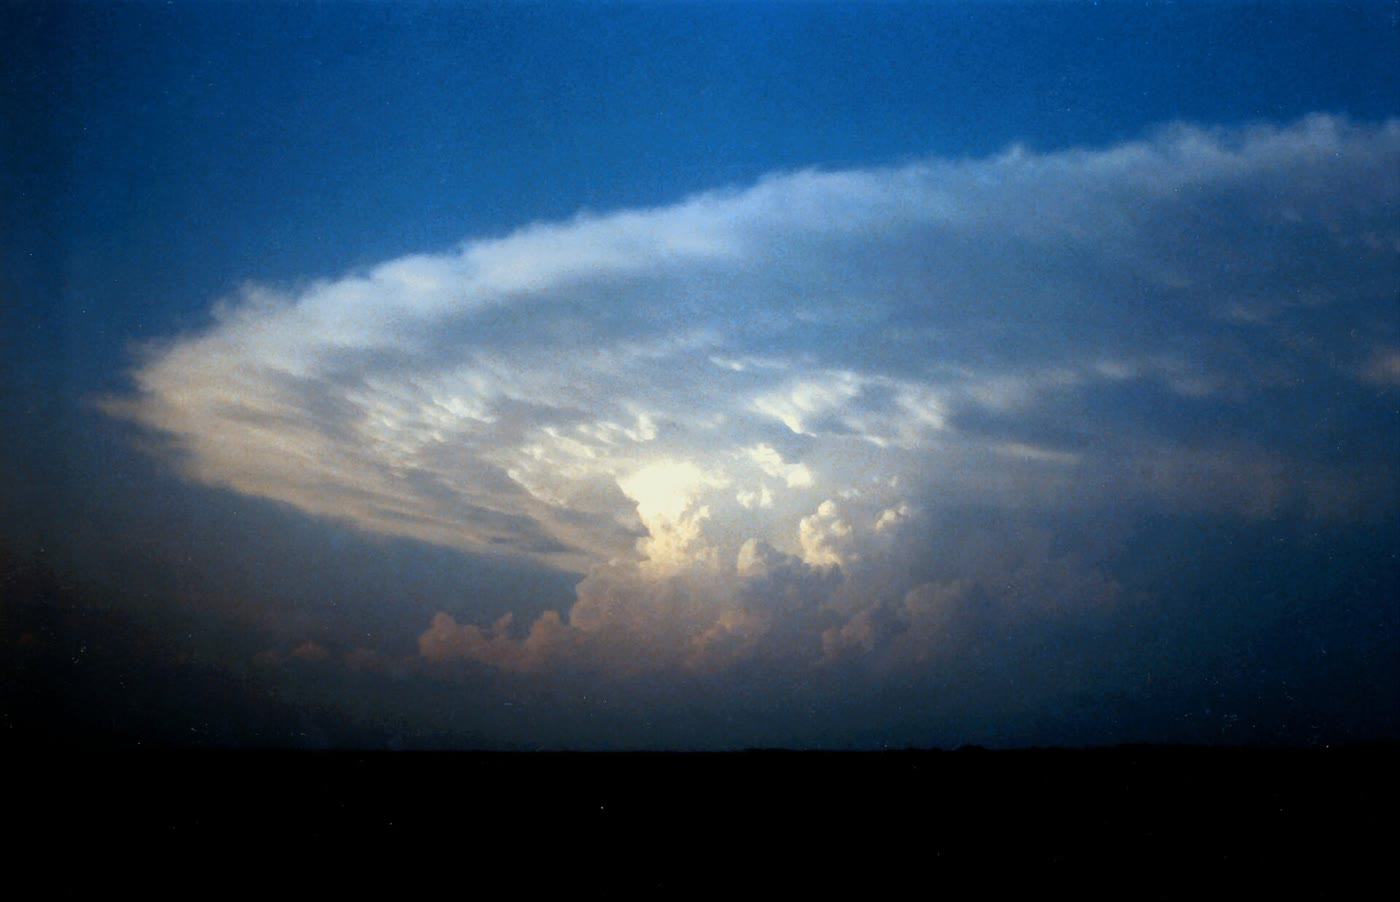
\includegraphics[width=0.6\linewidth]{images/book4/b2-21-supercell-anvil.jpg}
\par\smallskip{\small عاصفة رعدية فوق نبراسكا، 20 أبريل 1985: ينبسط تيّارها الصاعد في
سندان حيث يبلغ مستوى توازنه، قرب التروبوبوز. الصورة: \mbox{\textdir TLT Stephen Corfidi,
NOAA/NWS}، ملك عام، عبر \mbox{\textdir TLT Wikimedia Commons}.}
\end{omfigure}
% ledger: nws4:lfc-el

\section{فيزياء السحب الدقيقة}\label{sec:b2:atmospheric-thermodynamics:microphysics}

الطرد عند مستوى تكاثفه بالرفع مشبع فوق سطح مائي مستوٍ. لكنّ القطيرة ليست مستوية: فكتب
الفيزياء تبيّن أن الطور الجديد لا يظهر عند التوازن، بل عبر التنوّي وحده، وكتب
الكيمياء أن \omterm{def:b2:atmospheric-thermodynamics:moist-air}{ضغط البخار} فوق سطح منحنٍ يفوق ضغطه فوق سطح مستوٍ
(معادلة كلفن). ومع الثابت $A$ في \cref{prop:b2:atmospheric-thermodynamics:kohler}
أدناه، لا تكون قطيرة من الماء النقي قطرها \qty{2}{nm} في توازن إلا عند نسبة التشبّع
$\exp(2.1/2) = 2.9$، أي فوق تشبّع قدره \qty{190}{\percent}، أعلى بكثير من أجزاء الواحد في المئة
التي تتنشّط عندها الجسيمات: فالقطيرات تتكوّن على جسيمات.

\begin{definition}[فوق التشبّع؛ نواة التكاثف السحابية]\label{def:b2:atmospheric-thermodynamics:microphysics}
\emph{فوق التشبّع}\index{فوق التشبّع} للهواء هو $s = e/e_s - 1$، أي زيادة
ضغط بخاره على \omterm{def:b2:atmospheric-thermodynamics:moist-air}{ضغط البخار} المشبع فوق سطح مستوٍ من الماء النقي، ويُعطى عادة
بالنسبة المئوية. و\emph{نواة التكاثف السحابية}\index{نواة التكاثف السحابية} (CCN)
جسيم هبائي تتكوّن عليه قطيرة سحابية عند قيم فوق التشبّع الصغيرة في السحب.
وهي \emph{نواة التكاثف}\index{نواة التكاثف} في مجلّدات المدرسة.
\end{definition}
% ledger: nws4:ccn-bergeron, pk07:kohler, morrison20:processes

\begin{proposition}[منحنى كولر]\label{prop:b2:atmospheric-thermodynamics:kohler}
\index{منحنى كولر}
قطيرة محلول قطرها $D$ نمت على جسيم جاف قطره $D_d$ واسترطابيّته
$\kappa$ تكون في توازن مع نسبة التشبّع
\[
  S(D) = \frac{D^3 - D_d^3}{D^3 - D_d^3(1 - \kappa)}\,\exp\Bigl(\frac{A}{D}\Bigr), \qquad
  A = \frac{4\sigma M_w}{R T\rho_w},
\]
حيث $\sigma$ التوتّر السطحي و$\rho_w$ كثافة الماء (مسلَّم بها). ويُسمّى المنحنى $S(D)$
\emph{\omterm{prop:b2:atmospheric-thermodynamics:kohler}{منحنى كولر}}. ومن أجل $D \gg D_d$،
\[
  s = S - 1 \approx \frac{A}{D} - \frac{\kappa D_d^3}{D^3},
\]
الذي تبلغ قيمته العظمى عند القطر الحرج \omterm{def:b2:atmospheric-thermodynamics:microphysics}{وفوق التشبّع} الحرج
\[
  D_c = \sqrt{\frac{3\kappa D_d^3}{A}}, \qquad s_c = \sqrt{\frac{4A^3}{27\,\kappa D_d^3}} .
\]
\end{proposition}
% ledger: pk07:kohler

\begin{proof}[برهان التقريب]
الدالّة الأسّية هي عامل كلفن؛ والكسر هو نشاط الماء، وهو صيغة من قانون راؤول
يقيس فيها $\kappa$ مقدار الماء الذي تربطه المادّة المذابة. ومن أجل $D \gg D_d$
و$A \ll D$، يكون $\exp(A/D) \approx 1 + A/D$ والكسر $1 - \kappa D_d^3/D^3$ إلى الرتبة
الأولى؛ والجداء، إلى الرتبة الأولى، هو $1 + A/D - \kappa D_d^3/D^3$. وجعل المشتقّة
$-A/D^2 + 3\kappa D_d^3/D^4$ صفرًا يعطي $D_c^2 = 3\kappa D_d^3/A$، ثم $s_c = A/D_c -
A/(3D_c) = 2A/(3D_c)$، وهي الصيغة.
\end{proof}

مع $\sigma = \qty{0.072}{J/m^2}$ عند \qty{298.15}{K}، يكون $A = \qty{2.1}{nm}$. ولكبريتات الأمونيوم
$\kappa = 0.61$؛ وكلوريد الصوديوم أشدّ استرطابًا أيضًا ($\kappa = 1.28$)، وتقع معظم الجسيمات الجوية بين 0.1 و0.9.
وجسيم جاف من كبريتات الأمونيوم قطره \qty{50}{nm} له $D_c = \qty{0.33}{\micro m}$ و$s_c =
\qty{0.42}{\percent}$؛ وجسيم قطره \qty{100}{nm} له \qty{0.93}{\micro m} و\qty{0.15}{\percent}.
ويختلف التقريب عن القيمة العظمى الدقيقة بأقلّ من \qty{1}{\percent}.
% ledger: pk07:kohler, pk07:kappa

\begin{omfigure}
\centering
% figdata/bachelor-2/thermo.py part kohler
\begin{tikzpicture}
\begin{semilogxaxis}[width=0.72\linewidth, height=5.6cm, xmin=0.03, xmax=10, ymin=-0.4,
  ymax=1.1, xlabel={قطر القطيرة $D$ \babelsublr{(\unit{\micro m})}}, ylabel={فوق التشبّع $s$
  \babelsublr{(\unit{\percent})}}, tick label style={font=\scriptsize}, label style={font=\small},
  log ticks with fixed point, legend style={font=\scriptsize, draw=none, fill=none},
  legend pos=north east, legend cell align=left, unbounded coords=discard]
\addplot[ocBlue, thick, densely dotted] table[x=D_um, y=s30] {figdata/out/bachelor-2-thermo-kohler.dat};
\addlegendentry{$D_d = \qty{30}{nm}$}
\addplot[ocBlue, thick] table[x=D_um, y=s50] {figdata/out/bachelor-2-thermo-kohler.dat};
\addlegendentry{$D_d = \qty{50}{nm}$}
\addplot[ocBlue, thick, dashed] table[x=D_um, y=s100] {figdata/out/bachelor-2-thermo-kohler.dat};
\addlegendentry{$D_d = \qty{100}{nm}$}
\addplot[only marks, mark=*, mark size=1.5pt, black] coordinates {(0.1542,0.914) (0.3309,0.4244)
  (0.9345,0.1499)};
\draw[black!45] (axis cs:0.03,0) -- (axis cs:10,0);
\draw[ocRed, densely dashed] (axis cs:0.03,0.5) -- (axis cs:10,0.5);
\node[font=\scriptsize, ocRed, anchor=north west] at (axis cs:2.2,0.5) {$s = \qty{0.5}{\percent}$};
\end{semilogxaxis}
\end{tikzpicture}
\par\smallskip{\small منحنيات كولر لجسيمات من كبريتات الأمونيوم ($\kappa = 0.61$) بثلاثة أقطار
جافّة عند \qty{298.15}{K}، مع نقاطها الحرجة (النقاط). وفي هواء فوق تشبّعه \qty{0.5}{\percent}،
تنمو الجسيمات ذات \qty{50}{nm} و\qty{100}{nm} بلا حدّ؛ ويبقى
الجسيم ذو \qty{30}{nm} قطيرة غَبَش.}
\end{omfigure}
% ledger: pk07:kohler, pk07:kappa

يقسم المنحنى الجسيمات. فتحت قمّته تكون القطيرة في توازن مستقرّ: فإن نمت،
لم يعد الهواء فوق مشبع بما يكفي لها فتنكمش ثانية؛ وقطيرات الغَبَش هذه تنتفخ
وتنكمش مع الرطوبة. أمّا متى تجاوز فوق تشبّع الهواء $s_c$، فتصبح القطيرة
\emph{منشَّطة}: إذ تحتاج بعد القمّة إلى فوق تشبّع يتناقص باستمرار وهي تنمو، فتنمو
ما دام البخار موجودًا. والطرد الصاعد يبرد، فيرتفع فوق تشبّعه، وتتنشّط أكبر الجسيمات
وأكثرها ذوبانًا أوّلًا؛ ثم تأخذ القطيرات التي تصنعها البخار فتسقّف
\omterm{def:b2:atmospheric-thermodynamics:microphysics}{فوق التشبّع}. وفوق المحيطات النائية يوجد نحو 110 نوى تكاثف سحابية في كلّ سنتيمتر مكعّب نشطة
عند \qty{0.4}{\percent}، وفوق القارّات النائية قرابة ضعف ذلك، وفي الهواء الملوّث نحو
عشرة أضعاف. والماء نفسه حين يتوزّع على قطيرات أكثر يجعلها أصغر.
% ledger: andreae09:ccn, morrison20:processes

\begin{remark}[لماذا لا يصنع التكاثف وحده المطر]\label{rem:b2:atmospheric-thermodynamics:growth}
تنمو القطيرة بانتشار البخار نحوها. والتدفّق عبر كرة حول قطيرة
نصف قطرها $r$ هو $4\pi r D_v\,\Delta\rho_v$، حيث $D_v$ معامل انتشار البخار
و$\Delta\rho_v$ زيادة كثافة البخار بعيدًا عنها، فتنمو كتلتها $\tfrac43\pi r^3\rho_w$
بمعدّل يتناسب مع $r$: فيكون $r\,\mathrm{d}r/\mathrm{d}t$ ثابتًا وينمو $r^2$ خطّيًّا مع
الزمن. والقطيرات الكبيرة تنمو أبطأ من الصغيرة، والجماعة التي تنمو بالتكاثف
وحده تضيق ولا تتّسع. وتتكوّن قطرات المطر حين تتصادم قطيرات مختلفة الأحجام، تسقط
بسرعات مختلفة، فتلتحم.
\end{remark}
% ledger: morrison20:processes

فوق مستوى \qty{0}{\celsius} تتألّف السحابة من قطيرات فائقة التبريد حتى تبدأ جسيمات منوّية
للجليد بلورات جليدية. عندئذ يعمل فرق اللوحة اليمنى من
شكل التشبّع: فالهواء المشبع فوق القطيرات فوق مشبع بنسبة \qty{10}{\percent} فوق
الجليد عند \qty{-10}{\celsius}، أي عشرات أضعاف قيم \omterm{def:b2:atmospheric-thermodynamics:microphysics}{فوق التشبّع} التي تنشّطت عندها القطيرات.
وتنمو البلورات بالترسّب البخاري على حساب القطيرات، التي تتبخّر (عملية
برجيرون، أي آلية البلورات الجليدية في مجلّدات المدرسة)، وتجمع قطيرات تتجمّد
عليها (التصقيع).
% ledger: nws4:ccn-bergeron, morrison20:processes, iapws4:sublimation

\begin{omfigure}
\centering
\begin{tikzpicture}[font=\scriptsize, box/.style={draw=black!60, rounded corners=2pt,
  align=center, minimum height=0.95cm, text width=2.1cm, fill=#1}, box/.default=white,
  >=Stealth]
\node[anchor=west, black!60] at (-1.15,0.8) {عمليات دافئة};
\node[box=black!6] (ccn) at (0,0) {جسيم هبائي\\(CCN)};
\node[box=ocBlue!8] (haze) at (4.2,0) {قطيرة غَبَش\\$s < s_c$};
\node[box=ocBlue!15] (act) at (8.4,0) {قطيرة منشَّطة\\$s > s_c$};
\node[box=ocBlue!25] (rain) at (12.6,0) {قطرة مطر};
\draw[->] (ccn) -- node[above] {الرطوبة} (haze);
\draw[->] (haze) -- node[above] {الصعود} (act);
\draw[->] (act) -- node[above, align=center] {\foreignlanguage{arabic}{تصادم،}\\والتحام} (rain);
\node[anchor=west, black!60] at (-1.15,-3.4) {عمليات جليدية};
\node[box=black!6] (inp) at (0,-2.6) {جسيم منوٍّ\\للجليد};
\node[box=omMeth!10] (ice) at (4.2,-2.6) {بلّورة جليد\\\foreignlanguage{arabic}{تحت \mbox{\textdir TLT \qty{0}{\celsius}}}};
\node[box=omMeth!20] (snow) at (8.4,-2.6) {ثلج، بَرَد رخو};
\node[box=ocBlue!25] (rain2) at (12.6,-2.6) {مطر};
\draw[->] (inp) -- (ice);
\draw[->] (ice) -- node[above, align=center] {\foreignlanguage{arabic}{ترسّب بخاري،}\\تصقيع} (snow);
\draw[->] (snow) -- node[above] {الانصهار} (rain2);
\draw[->, omMeth!60!black, dashed] (act.south) -- node[pos=0.45, right=4pt, align=left,
  omMeth!60!black] {بخار من\\القطيرات المتبخّرة} (ice.north);
\end{tikzpicture}
\par\smallskip{\small الطريقان من البخار إلى الهطول: تنشّط القطيرات ونموّها،
ثم التصادم والالتحام (في الأعلى)؛ وبلّورات جليد تنمو على حساب القطيرات
فائقة التبريد، وتتصقّع، وتنصهر وهي تسقط في هواء أدفأ (في الأسفل).}
\end{omfigure}
% ledger: morrison20:processes, nws4:ccn-bergeron

\begin{inthefield}[إطلاق صباحي]
\begin{minipage}[t]{0.54\linewidth}\vspace{0pt}
في كلّ محطّة لرصد طبقات الجوّ العليا يجهّز الفنّي المنطاد والمسبار اللاسلكي في الساعة
التي تسبق الساعتين 00 و12 بالتوقيت العالمي المنسّق، وهما الموعدان اللذان ترصد فيهما أكثر من ثمانمئة محطّة في العالم
معًا. ويتدلّى الجهاز، الذي تتراوح كتلته من 60 إلى \qty{80}{g}، تحت المنطاد ويرسل الضغط
والحرارة والرطوبة وموقعه الساتلي كلّ ثانية. ويرتفع المنطاد نحو
\qty{300}{m} في الدقيقة، مدّة ساعتين أو أكثر، متجاوزًا \qty{35}{km} قبل أن ينفجر، وقد ينجرف
أكثر من \qty{300}{km}. ويرسم المتنبّئون المقطع على \omterm{def:b2:atmospheric-thermodynamics:diagram}{المخطّط المائل}، وفي
الأيام التي يُتوقّع فيها طقس عنيف تطلق بعض المحطّات مناطيد إضافية.
\end{minipage}\hfill
\begin{minipage}[t]{0.42\linewidth}\vspace{0pt}
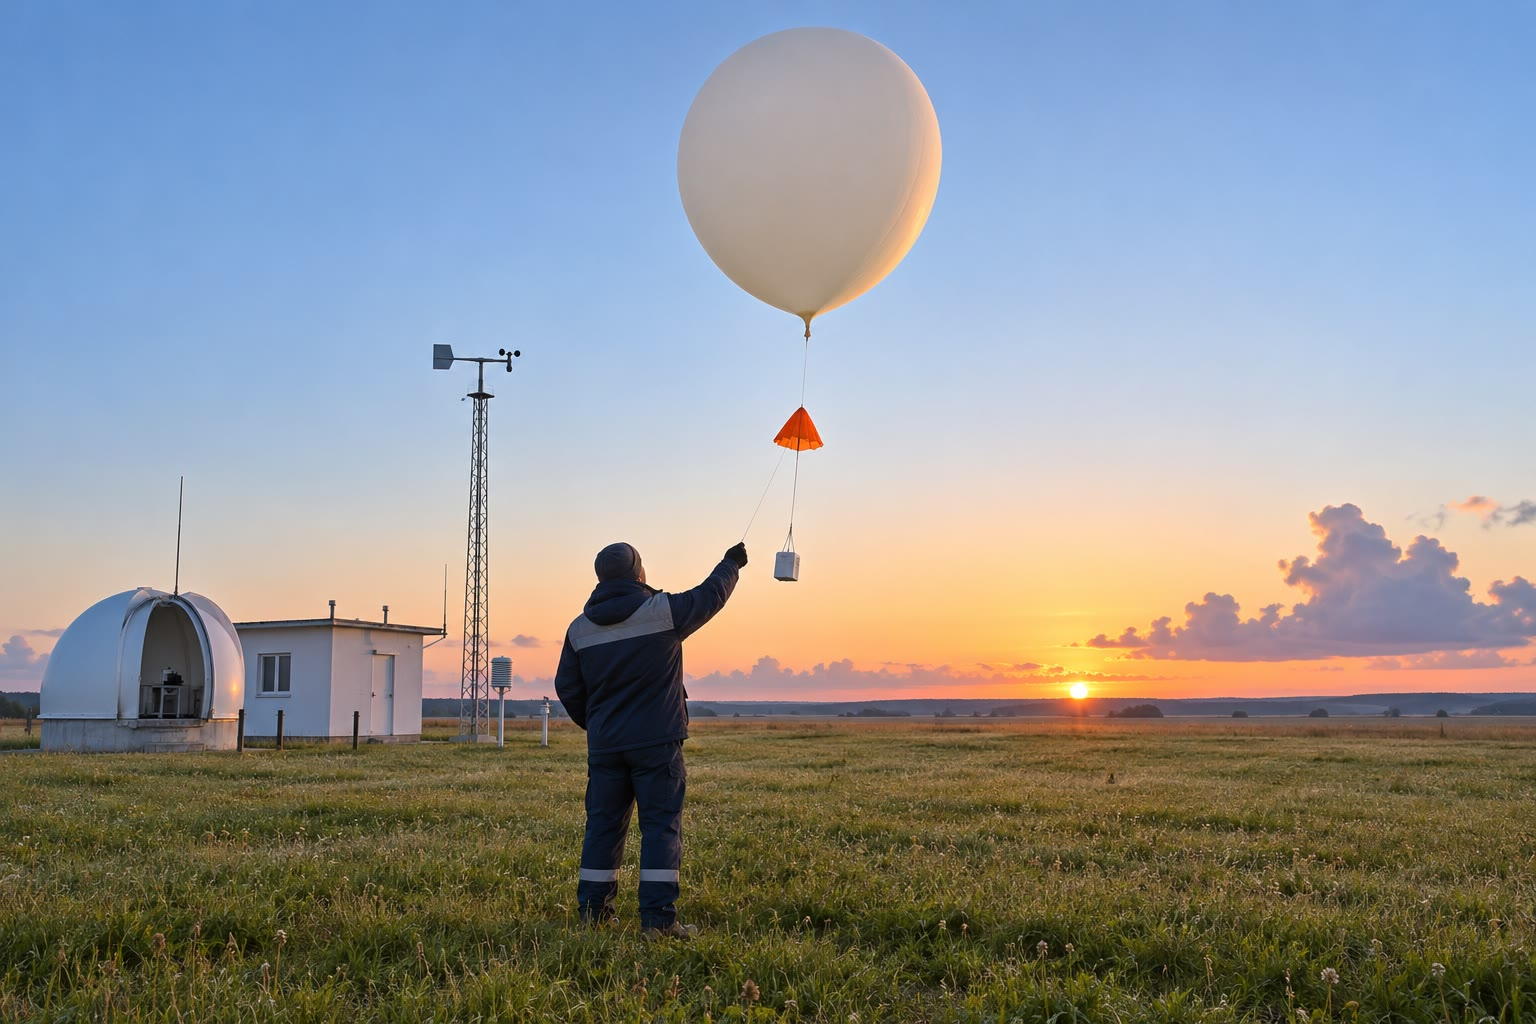
\includegraphics[width=\linewidth]{images/book4/ai/b2-radiosonde-launch.jpg}

{\scriptsize مسبار لاسلكي يُطلق عند الفجر من محطّة أرصاد (رسم توضيحي مولَّد
بالذكاء الاصطناعي).}
\end{minipage}
% ledger: nws:radiosonde, nws4:upperair
\end{inthefield}

\section*{التمارين}\label{sec:b2:atmospheric-thermodynamics:exercises}

معطيات التمارين، ما لم يُذكر غير ذلك: $e_s(T) = \qty{6.117}{hPa} \times
\exp[\qty{5419}{K} \times (1/\qty{273.16}{K} - 1/T)]$؛ و$\varepsilon = 0.622$، و$R_d =
\qty{287.0}{J.kg^{-1}.K^{-1}}$، و$R_v = \qty{461.5}{J.kg^{-1}.K^{-1}}$، و$c_p =
\qty{1004.5}{J.kg^{-1}.K^{-1}}$، و$L = \qty{2.501e6}{J/kg}$، و$g = \qty{9.81}{m.s^{-2}}$،
و$\Gamma_d = \qty{9.8}{K/km}$.
% ledger: nist4:water-sat, iapws4:sublimation, const:R, earth:Mmol, nist4:water-mw, nasa:grc-gamma

\begin{exercise}[$\star$]\label{exo:b2:atmospheric-thermodynamics:1}
عند \qty{850}{hPa} تبلغ درجة الحرارة \qty{10.0}{\celsius} ونقطة الندى \qty{5.0}{\celsius}.
(أ) أوجد \omterm{def:b2:atmospheric-thermodynamics:moist-air}{ضغط البخار} \omterm{def:b2:atmospheric-thermodynamics:moist-air}{وضغط البخار} المشبع. (ب) أوجد الرطوبة النسبية.
(ج) أوجد \omterm{def:b2:atmospheric-thermodynamics:moist-air}{نسبة الخلط} \omterm{def:b2:atmospheric-thermodynamics:moist-air}{والرطوبة النوعية}، بالغرامات لكل كيلوغرام.
\end{exercise}

\begin{exercise}[$\star$]\label{exo:b2:atmospheric-thermodynamics:2}
(أ) بكم في المئة لكل كلفن يرتفع $e_s$ عند \qty{0}{\celsius} و\qty{20}{\celsius}
و\qty{30}{\celsius}؟ (ب) احسب $e_s$ عند \qty{20}{\celsius} وعند \qty{25}{\celsius}،
ونسبتهما؛ وقارن بالقيمة $1.063^5$. (ج) القيمة المقيسة عند \qty{20}{\celsius} هي
\qty{23.39}{hPa}. بكم تخطئ الصيغة، وفي أيّ اتجاه؟ ولماذا؟
\end{exercise}
% ledger: nist4:water-sat

\begin{exercise}[$\star$]\label{exo:b2:atmospheric-thermodynamics:3}
عند الظهر يكون هواء السطح عند \qty{30}{\celsius} ونقطة نداه \qty{14}{\celsius}. (أ) على
أيّ ارتفاع فوق الأرض تتكوّن قواعد السحب الركامية؟ (ب) ما درجة حرارة طرد
هناك، وفق المنحنى الأديباتي الجاف؟ (ج) ما نقطة نداه هناك، مع $\Gamma_{\text{ندى}} =
\qty{1.8}{K/km}$؟ علّق. (د) لاحقًا يسخن الهواء إلى \qty{33}{\celsius}، مع بقاء نقطة الندى
على حالها. أين قواعد السحب الآن؟
\end{exercise}

\begin{exercise}[$\star$]\label{exo:b2:atmospheric-thermodynamics:4}
اقرأ \omterm{def:b2:atmospheric-thermodynamics:diagram}{المخطّط المائل} لسبر نورمان. (أ) حتى أيّ ضغط يكون الهواء قرب
الأرض مشبعًا، أو قريبًا من التشبّع؟ (ب) أين الانعكاس الحراري، وكيف يظهر؟ (ج) اقرأ
\omterm{def:b2:atmospheric-thermodynamics:lcl}{مستوى التكاثف بالرفع} \omterm{def:b2:atmospheric-thermodynamics:parcel-levels}{ومستوى الحمل الحرّ} \omterm{def:b2:atmospheric-thermodynamics:parcel-levels}{ومستوى التوازن} لطرد السطح. (د) كيف تتقارن نقطة الندى ودرجة الحرارة
فوق الانعكاس مباشرة، وماذا يقول ذلك عن هذا الهواء؟
\end{exercise}
% ledger: data:b4-sounding

\begin{exercise}[$\star\star$]\label{exo:b2:atmospheric-thermodynamics:5}
لهواء مداري عند \qty{1000}{hPa} القيمتان $T = \qty{30.0}{\celsius}$ و$r = \qty{20}{g/kg}$. (أ) أوجد
درجة حرارته الافتراضية بدقّة وبالتقريب $T(1 + 0.61\,r)$. (ب) أوجد كثافتَي
هذا الهواء والهواء الجاف عند درجة الحرارة والضغط نفسيهما. (ج) بكم يجب أن يُسخَّن الهواء الجاف
ليصبح بالخفّة نفسها؟ (د) لماذا يهمّ هذا في الحمل فوق البحار الدافئة؟
\end{exercise}

\begin{exercise}[$\star\star$]\label{exo:b2:atmospheric-thermodynamics:6}
استعمل \cref{prop:b2:atmospheric-thermodynamics:gamma-s} عند \qty{1000}{hPa}، مع $r_s$ من
\cref{prop:b2:atmospheric-thermodynamics:humidity}. (أ) احسب $r_s$ و$\Gamma_s$ عند
\qty{0}{\celsius} و\qty{20}{\celsius} و\qty{30}{\celsius}. (ب) بكم يكون طرد مشبع عند \qty{20}{\celsius} أدفأ من طرد
جاف بعد صعود \qty{1}{km}، إن بقي معدّل انخفاضه
ثابتًا؟ (ج) لماذا يتقلّص الفرق في الأعالي؟
\end{exercise}

\begin{exercise}[$\star\star$]\label{exo:b2:atmospheric-thermodynamics:7}
لطرد السطح في نورمان ($p = \qty{971.1}{hPa}$، $T = \qty{19.0}{\celsius}$، $T_d =
\qty{18.5}{\celsius}$) مستوى تكاثف بالرفع عند \qty{18.35}{\celsius}. (أ) احسب نسبة خلطه،
ودرجة حرارته الكامنة \omterm{def:b2:atmospheric-thermodynamics:theta-e}{ودرجة حرارته الكامنة المكافئة}. (ب) حين يُرفع، يكون عند
\qty{-8.9}{\celsius} عند \qty{500}{hPa}، مشبعًا. احسب $\theta$ و$\theta_e$ له هناك.
(ج) أيّهما محفوظة؟
\end{exercise}
% ledger: data:b4-sounding

\begin{exercise}[$\star\star$]\label{exo:b2:atmospheric-thermodynamics:8}
طرد أدفأ من محيطه بمقدار \qty{4}{K} بين \qty{700}{hPa}، مستوى حمله الحرّ،
و\qty{300}{hPa}، مستوى توازنه؛ أهمل تصحيح الحرارة الافتراضية. (أ) احسب CAPE له. (ب)
احسب $w_{\max}$. (ج) في أيّ فئة تقع CAPE هذه؟ (د) على \omterm{def:b2:atmospheric-thermodynamics:diagram}{المخطّط المائل}، ما
شكل المساحة الموجبة، ولماذا تساوي مساحتها ما حُسب؟
\end{exercise}
% ledger: hgx:cape

\begin{exercise}[$\star\star$]\label{exo:b2:atmospheric-thermodynamics:9}
خذ $A = \qty{2.1}{nm}$ وكبريتات الأمونيوم، $\kappa = 0.61$. (أ) أوجد القطر الحرج
\omterm{def:b2:atmospheric-thermodynamics:microphysics}{وفوق التشبّع} الحرج لجسيم جاف قطره \qty{80}{nm}. (ب) ما أصغر جسيم جاف
يتنشّط في هواء فوق تشبّعه \qty{0.3}{\percent}؟ وعند \qty{0.1}{\percent}؟ (ج) يرفع تيّار صاعد
\omterm{def:b2:atmospheric-thermodynamics:microphysics}{فوق التشبّع} من \qty{0.1}{\percent} إلى \qty{0.3}{\percent}: ماذا يحدث
لعدد القطيرات، ولحجمها مع الكمّية نفسها من الماء السائل؟
\end{exercise}
% ledger: pk07:kappa, pk07:kohler

\begin{exercise}[$\star\star\star$]\label{exo:b2:atmospheric-thermodynamics:10}
كان لطرد السطح في نورمان كبح حمل قدره نحو \qty{-130}{J/kg} \omterm{def:b2:atmospheric-thermodynamics:virtual}{بدرجة الحرارة الافتراضية}.
(أ) بأيّ سرعة رأسية يجب أن يغادر الأرض ليبلغ مستوى حمله الحرّ بزخمه
وحده؟ (ب) قمّة الانعكاس عند \qty{889.1}{hPa} و\qty{20.5}{\celsius}. إلى أيّ
درجة حرارة يجب أن يسخن هواء السطح عند \qty{971.1}{hPa} كي لا يكون طرد مرفوع رفعًا أديباتيًّا
جافًّا أبرد من قمّة الانعكاس؟ (ج) لو بقيت نقطة نداه عند
\qty{18.5}{\celsius}، فأين تكون قاعدة سحابته؟ (د) اذكر طريقتين يزيل بهما الغلاف الجوي
مثل هذا الغطاء دون الشمس.
\end{exercise}
% ledger: data:b4-sounding, nws4:cin

\begin{exercise}[$\star\star\star$]\label{exo:b2:atmospheric-thermodynamics:11}
(أ) بيّن من \cref{prop:b2:atmospheric-thermodynamics:gamma-s} أن $\Gamma_s \to \Gamma_d$
حين $r_s \to 0$. (ب) بيّن أنه حين $Lr_s/(R_dT) \gg 1$، يكون $\Gamma_s \to gR_vT/(LR_d)$،
واحسبه عند \qty{303}{K}. (ج) قارن بالمعدّل $\Gamma_{\text{ندى}}$ في
\cref{prop:b2:atmospheric-thermodynamics:lcl} حين $T_d = T$، وفسّر لماذا تتطابق
النهايتان. (د) هل تُبلغ نهاية (ب) في الغلاف الجوي؟ استعمل القيمة $\Gamma_s =
\qty{3.4}{K/km}$ عند \qty{30}{\celsius} و\qty{1000}{hPa}.
\end{exercise}

\begin{exercise}[$\star\star\star$]\label{exo:b2:atmospheric-thermodynamics:12}
فوق الماء فائق التبريد وفوق الجليد يبلغ ضغطا البخار المشبع 2.868
و\qty{2.599}{hPa} عند \qty{-10}{\celsius}، و1.257 و\qty{1.032}{hPa} عند \qty{-20}{\celsius}.
(أ) أوجد \omterm{def:b2:atmospheric-thermodynamics:microphysics}{فوق التشبّع} بالنسبة إلى الجليد لهواء مشبع فوق الماء عند كلتا الدرجتين. (ب)
قارن بقيم \omterm{def:b2:atmospheric-thermodynamics:microphysics}{فوق التشبّع} التي تتنشّط عندها القطيرات. (ج) فسّر لماذا تتحوّل سحابة من
قطيرات فائقة التبريد تتلقّى بضع بلّورات جليد إلى جليد. (د) لماذا يكون الأثر
أضعف قرب \qty{0}{\celsius}؟
\end{exercise}
% ledger: iapws4:sublimation, su26:svp, nws4:ccn-bergeron

\begin{problem}[{مسألة نهاية الأسبوع --- قراءة السبر الصباحي}]\label{pb:b2:atmospheric-thermodynamics:1}
يعطي الجدول سبر نورمان، أوكلاهوما، عند الساعة 12 بالتوقيت العالمي المنسّق في 16 أبريل 2026، عند المستويات المستعملة
هنا: الضغط، والارتفاع فوق مستوى البحر، ودرجة الحرارة، ونقطة الندى، ودرجة حرارة
طرد السطح مرفوعًا كما في \cref{met:b2:atmospheric-thermodynamics:lift}، محسوبة
بمكاملة \cref{prop:b2:atmospheric-thermodynamics:gamma-s} بخطوات صغيرة. ويسجّل السبر
التروبوبوز عند \qty{235.3}{hPa} و\qty{10954}{m}. استعمل معطيات التمارين
ودرجات الحرارة (لا درجات الحرارة الافتراضية) ما لم يُطلب غير ذلك.

\begin{center}
\small
\begin{tabular}{rrrrr}
\hline
\mbox{\textdir TLT $p$ (\unit{hPa})} & \mbox{\textdir TLT $z$ (\unit{m})} & \mbox{\textdir TLT $T$ (\unit{\celsius})} & \mbox{\textdir TLT $T_d$ (\unit{\celsius})} &
\mbox{\textdir TLT $T_{\text{طرد}}$ (\unit{\celsius})} \\
\hline
971.1 & 345 & 19.0 & 18.5 & 19.0 \\
925.0 & 763 & 17.3 & 17.3 & 16.9 \\
907.7 & 924 & 16.4 & 16.4 & 16.2 \\
889.1 & 1102 & 20.5 & 9.5 & 15.4 \\
850.0 & 1489 & 18.6 & $-1.8$ & 13.7 \\
700.0 & 3110 & 4.5 & $-12.2$ & 6.1 \\
500.0 & 5725 & $-18.4$ & $-36.6$ & $-8.9$ \\
400.0 & 7357 & $-30.4$ & $-55.6$ & $-20.4$ \\
300.0 & 9349 & $-42.7$ & $-66.3$ & $-37.1$ \\
250.0 & 10560 & $-49.8$ & $-69.8$ & $-48.3$ \\
200.0 & 12006 & $-52.3$ & $-78.3$ & $-61.8$ \\
\hline
\end{tabular}
\end{center}

\medskip\noindent\textbf{الجزء الأول --- الهواء قرب الأرض.}
\begin{enumerate}
  \item أوجد ضغط بخار هواء السطح، إلى منزلة عشرية واحدة.
  \item أوجد نسبة خلطه، إلى منزلة عشرية واحدة.
  \item أوجد رطوبته النوعية.
  \item أوجد رطوبته النسبية.
  \item بكم تتجاوز درجة حرارته الافتراضية درجة حرارته؟
  \item أوجد ارتفاع مستوى تكاثفه بالرفع فوق الأرض بقاعدة \qty{125}{m}، والضغط
        هناك (خذ للطبقة درجة حرارة افتراضية متوسطة قدرها \qty{294.7}{K}).
  \item أوجد درجة حرارته الكامنة.
\end{enumerate}

\medskip\noindent\textbf{الجزء الثاني --- الغطاء والطبقات التي فوقه.}
\begin{enumerate}[resume]
  \item عند \qty{925}{hPa}، هل الطرد أدفأ من محيطه أم أبرد، وبكم؟
  \item أوجد معدّل الانخفاض بين 907.7 و\qty{889.1}{hPa}. أيّ نوع من الطبقات هذه؟
  \item بكم يكون الطرد أبرد من محيطه عند \qty{889.1}{hPa}؟
  \item أوجد الرطوبة النسبية عند \qty{850}{hPa}. من أين يمكن أن يكون هذا الهواء قد أتى؟
  \item أوجد معدّل الانخفاض المتوسط بين 850 و\qty{500}{hPa} وصنّف الطبقة.
  \item أوجد مؤشّر الرفع وفئته.
\end{enumerate}

\medskip\noindent\textbf{الجزء الثالث --- الطاقة.}
\begin{enumerate}[resume]
  \item احسب الزيادة $\Delta T = T_{\text{طرد}} - T$ عند كلّ مستوى من الجدول.
  \item أوجد \omterm{def:b2:atmospheric-thermodynamics:parcel-levels}{مستوى الحمل الحرّ} باستيفاء $\Delta T$ خطّيًّا بدلالة $\ln p$، إلى أقرب هكتوباسكال،
        وارتفاعه باستيفاء $z$ بالطريقة نفسها.
  \item أوجد \omterm{def:b2:atmospheric-thermodynamics:parcel-levels}{مستوى التوازن} وارتفاعه بالطريقة نفسها. وقارن بالتروبوبوز.
  \item احسب CAPE بقاعدة شبه المنحرف بدلالة $\ln p$، من \omterm{def:b2:atmospheric-thermodynamics:parcel-levels}{مستوى الحمل الحرّ} إلى \omterm{def:b2:atmospheric-thermodynamics:parcel-levels}{مستوى التوازن} مرورًا
        بمستويات الجدول.
  \item في أيّ فئة تقع؟
  \item احسب \omterm{def:b2:atmospheric-thermodynamics:cape}{كبح الحمل} بالطريقة نفسها، من الأرض إلى \omterm{def:b2:atmospheric-thermodynamics:parcel-levels}{مستوى الحمل الحرّ}.
  \item يعطي حساب على شبكة خطوتها \qty{1}{hPa} قيمة CAPE قدرها \qty{2100}{J/kg} بدرجات
        الحرارة و\qty{2230}{J/kg} بدرجات الحرارة الافتراضية. لماذا تختلف القيم
        الثلاث؟
\end{enumerate}

\medskip\noindent\textbf{الجزء الرابع --- العاصفة التي يستطيع الهواء تغذيتها.}
\begin{enumerate}[resume]
  \item ما السرعة الرأسية التي تعطيها نظرية الطرد بقيمة CAPE في السؤال 17؟
  \item بنصف تلك السرعة طوال الطريق، كم يستغرق الهواء ليصعد من \omterm{def:b2:atmospheric-thermodynamics:parcel-levels}{مستوى الحمل الحرّ} إلى \omterm{def:b2:atmospheric-thermodynamics:parcel-levels}{مستوى التوازن}؟
  \item اذكر أثرين يجعلان التيّار الصاعد الحقيقي أبطأ.
  \item خلاصة القول: ما سرعة التيّار الصاعد التي تتنبّأ بها نظرية الطرد لعاصفة يغذّيها
        هواء السطح هذا الصباح؟
\end{enumerate}
\end{problem}
% ledger: data:b4-sounding, hgx:cape, nws4:lifted-index, nws4:cape
